% !Mode:: "TeX:UTF-8"
\documentclass[fancyhdr,adobefonts,oneside,hyperref,openany,a4paper,UTF8]{ctexbook}
\usepackage{py-book}
\usepackage{code-listing}
\usepackage{theorem}
\usepackage{highlight}
\usepackage{lipsum}
\usepackage{calc}


%---------------------------------------
\author{Pythonee}
\title{书籍标题}
\date{2014-04-23}
\homepage{py-note.appspot.com}
\email{pythonee@gmail.com}
\claimcopyright{随意使用\ 任意修改}
%---------------------------------------

\makeindex
\usepackage[totoc]{idxlayout}   % add index to table of contents


\begin{document}
\maketitle

%---------------------------------------

\frontmatter
\pdfbookmark{目录}{toc}	% 把目录添加到书签
\tableofcontents
\listoftables
\listoffigures
\lstlistoflistings
\setcounter{page}{0}
\chapter{摘要}
\lipsum[1]
\chapter{序}
\lipsum[1]


%---------------------------------------

\mainmatter
\part{我爱\TeX}
\chapter{简单介绍}
\lipsum

\part{我的 \LaTeX 模板}
\chapter{插入图片}

\begin{figure}[htp]
  \centering
    
\includegraphics[scale=0.25]{img/tiger}
    \caption{基本插入技巧}
    \label{fig:tiger}
\end{figure}

\section{基本插入技巧}


\begin{figure}[htp]
  \centering
    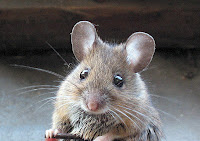
\includegraphics[width=0.2\textwidth,height=2.5cm]{img/mouse}~
    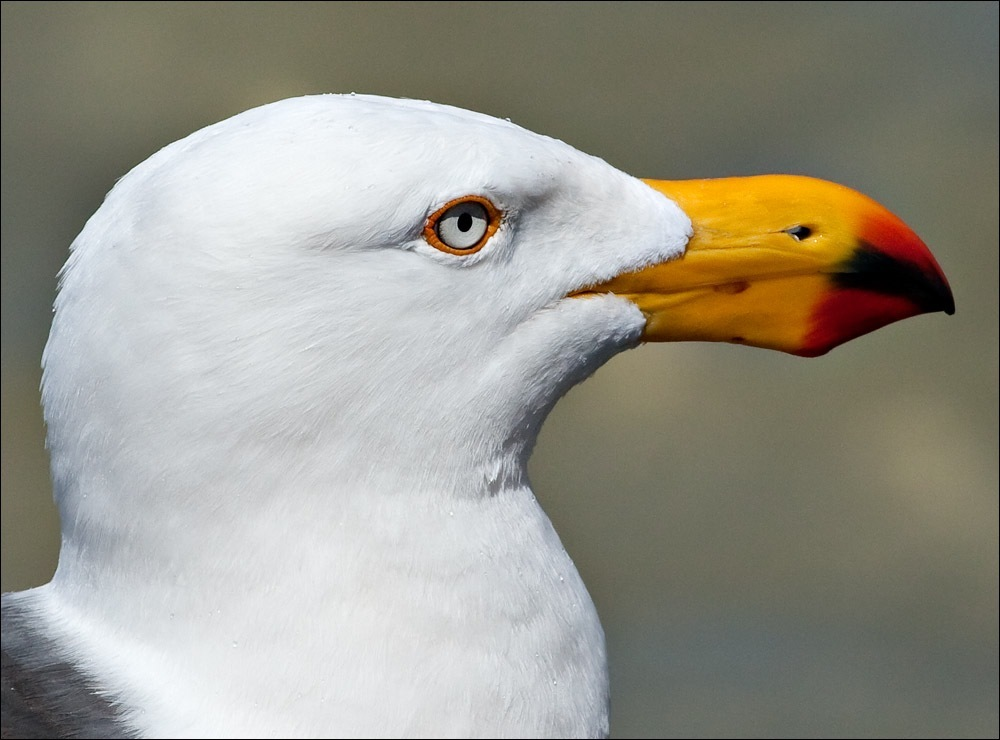
\includegraphics[width=0.2\textwidth,height=2.5cm]{img/gull}~
    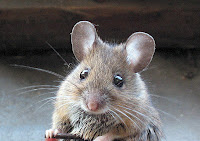
\includegraphics[width=0.2\textwidth,height=2.5cm]{img/mouse}
    \caption{多图片并排}
    \label{fig:tiger}
\end{figure}

\begin{figure}[htp]
    \centering
    \subfigure[First caption]
    {
        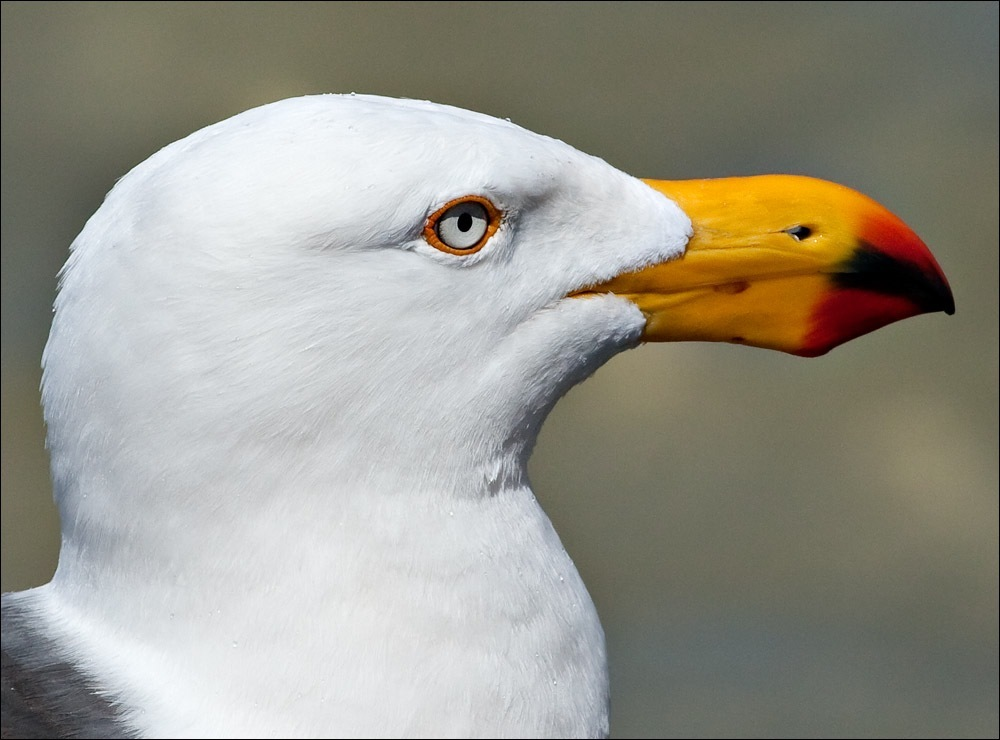
\includegraphics[width=1.0in,height=2cm]{img/gull}
        \label{fig:first_sub}
    }
    \\
    \subfigure[Second caption]
    {
        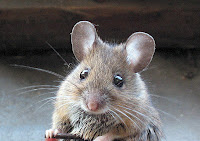
\includegraphics[width=1.0in,height=2cm]{img/mouse}
        \label{fig:second_sub}
    }
    \subfigure[Third caption]
    {
        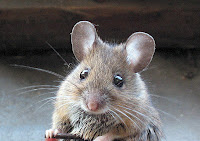
\includegraphics[width=1.0in,height=2cm]{img/mouse}
        \label{fig:third_sub}
    }
    \caption{subfigure的使用}
    \label{fig:sample_subfigures}
\end{figure}

\section{测试计数器}

\begin{SCfigure}
  \centering
  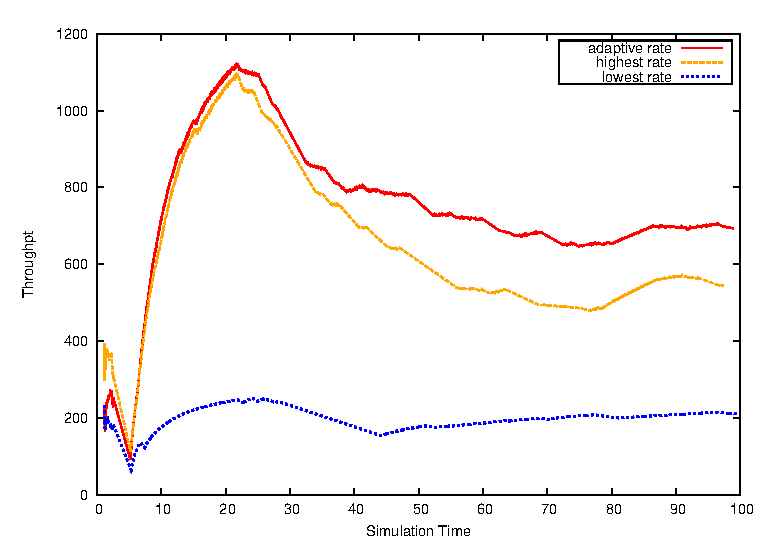
\includegraphics[width=0.5\textwidth]{img/throughput}
  \caption{ 边注标题}
\end{SCfigure}




It happens that you'll generate figures with too much (or too little) white space on the top or bottom. In such a case, you can simply make use of the optional argument [lineheight]. It specifies the height of the figure in number of lines of text. Also remember that the environment center adds some extra white space at its top and bottom;

It happens that you'll generate figures with too much (or too little) white space on the top or bottom. In such a case, you can simply make use of the optional argument [lineheight]. It specifies the height of the figure in number of lines of text. Also remember that the environment center adds some extra white space at its top and bottom;

\begin{wrapfigure}{r}{0.5\textwidth}
  \vspace{-20pt}
  \begin{center}
    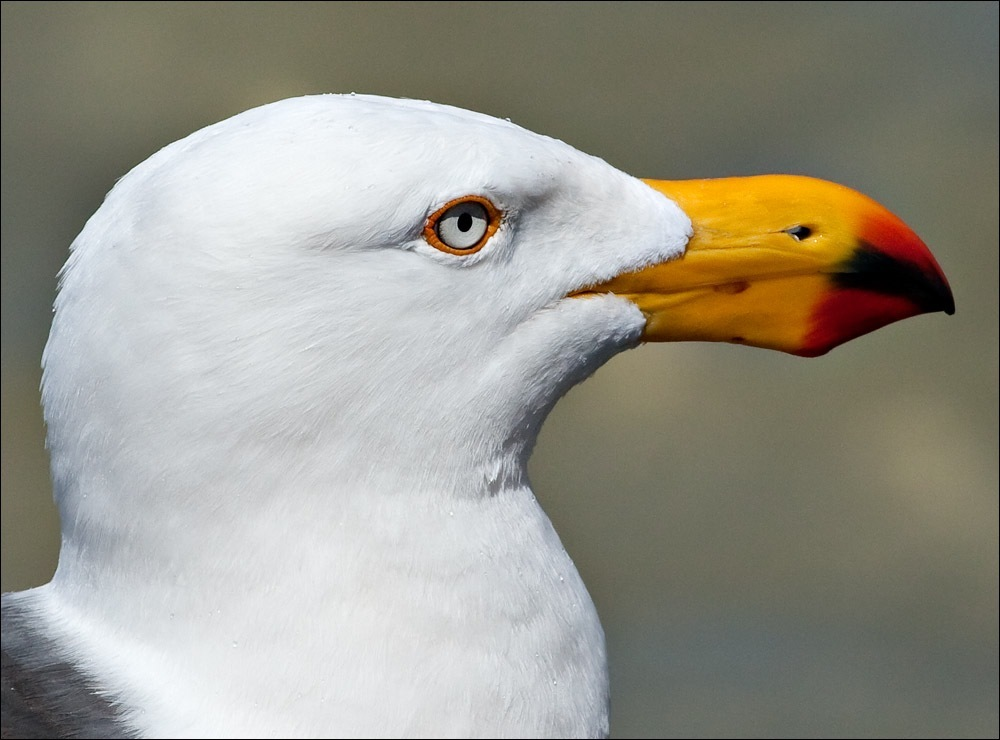
\includegraphics[width=0.48\textwidth]{img/gull}
  \end{center}
  \vspace{-20pt}
  \caption{图片环绕}
  \vspace{-10pt}
\end{wrapfigure}
It happens that you'll generate figures with too much (or too little) white space on the top or bottom. In such a case, you can simply make use of the optional argument [lineheight]. It specifies the height of the figure in number of lines of text. Also remember that the environment center adds some extra white space at its top and bottom;
It happens that you'll generate figures with too much (or too little) white space on the top or bottom. In such a case, you can simply make use of the optional argument [lineheight]. It specifies the height of the figure in number of lines of text. Also remember that the environment center adds some extra white space at its top and bottom;

\chapter{插入表格}
\section{常见表格}

\begin{table}[htp]
\centering
\caption{\label{tab:multicolumn}多行多列表格}
\begin{tabular}{|l|l|l|}
\hline
\multicolumn{3}{|c|}{Team Sheat} \\
\hline
Goalkeeper & GK & Paul Robinson \\
\hline
\multirow{4}{*}{Defenders} & LB & Lucus Radebe \\ & DC & Michael Duberry \\ & DC & Dominic Matteo \\ & RB & Didier Domi \\
\hline
\multirow{3}{*}{Midfielders} & MC & David Batty \\ & MC & Eirik Bakke \\ & MC & Jody Morris \\
\hline
Forward & FW & Jamie McMaster \\
\hline
\multirow{2}{*}{Strikers} & ST & Alan Smith \\ & ST & Mark Viduka \\
\hline
\end{tabular}
\end{table}

\begin{table}[htp]
\centering
\caption{\label{tab:mvat}@ 表达式}
\begin{tabular}{|r@{.}l|}
    \hline
    3&14159\\
    \hline
    16&2\\
    \hline
    123&456\\
    \hline
\end{tabular}
\end{table}

\begin{table}[htp]
\centering
\caption{\label{tab:diagonal }单元格对角线}
\begin{tabular}{|l|l|l|}
    \hline
    \multicolumn{2}{|c|}{\backslashbox{a}{b}} & c \\
    \hline
    d & e & f \\
    \hline
\end{tabular}
\end{table}

\section{复杂表格}

\begin{table}[htp]
   \begin{center}
   \caption{\label{tab:complicate}合并多行多列}
\begin{tabular}{l l l l l l l l }

\hline
\multicolumn{2}{l}{SAF 2507 stainless steel} & \multicolumn{6}{l}{($E$, $\nu$, $\sigma_y$, $n$)=(200 GPa, 0.3, 675 MPa, 0.19) } \\
\hline
  Friction coefficient
  & \multicolumn{3}{c}{H (GPa)} & \multicolumn{4}{c}{E (GPA) } \\
  \cline{2-8}
   & {O \& P} & {FEM} & {Diff (\%)} & {O \& P} & {Err(\%)} & {FEM} & {Err(\%)}  \\
  \cline{2-8}
\multicolumn{8}{l}{Conical indenter ($\theta =63.14^\circ $ )} \\
  $\mu$=0.0  & 4.23 & 3.60 & 0     & 230 & 14.99 & 210 & 5.00   \\
  $\mu$=0.05 & 4.23 & 3.73 & 3.61  & 230 & 14.99 & 213 & 6.50 \\
  $\mu$=0.1  & 4.23 & 3.80 & 5.56  & 230 & 14.99 & 216 & 8.00 \\
  $\mu$=0.15 & 4.23 & 3.88 & 7.78  & 230 & 14.99 & 218 & 9.00 \\
  $\mu$=0.3  & 4.23 & 3.99 & 10.83 & 230 & 14.99 & 221 & 10.50 \\
  $\mu$=0.6  & 4.23 & 3.99 & 10.83 & 230 & 14.99 & 221 & 10.50 \\
  $\mu$=1.0  & 4.23 & 3.99 & 10.83 & 230 & 14.99 & 221 & 10.50 \\
\hline
\multicolumn{8}{l}{Spherical indenter} \\
   $\mu$=0.0  & 3.84 & 3.43 & 0    & 218 & 8.95 & 206 & 3.00 \\
   $\mu$=0.05 & 3.84 & 3.49 & 1.75 & 218 & 8.95 & 208 & 4.00 \\
   $\mu$=0.1  & 3.84 & 3.57 & 4.08 & 218 & 8.95 & 210 & 5.00 \\
   $\mu$=0.15 & 3.84 & 3.62 & 5.54 & 218 & 8.95 & 212 & 6.00 \\
   $\mu$=0.3  & 3.84 & 3.66 & 6.71 & 218 & 8.95 & 213 & 6.50 \\
   $\mu$=0.6  & 3.84 & 3.66 & 6.71 & 218 & 8.95 & 213 & 6.50 \\
   $\mu$=1.0  & 3.84 & 3.66 & 6.71 & 218 & 8.95 & 213 & 6.50 \\
\hline
\end{tabular}
\end{center}
\end{table}


\chapter{插入代码}

\begin{withBookCaptionBlock}[caption=C语言代码,language={[ISO]C++},style=proBookStyle]
using namespace std;
int main(void)
{
    // %* \textit{创建一个简单的程序}  *)
    std::cout << "hello" << endl; // sample code $\alpha$
    return 0;
}
\end{withBookCaptionBlock}


\begin{originalCaptionBlock}[caption=伪代码,style=cleanStyle,language=C,frame=tb]
for i:=maxint to 0 do
begin
{ do nothing }
end;
Write(’Case insensitive ’);
Write(’Pascal keywords.’);
\end{originalCaptionBlock}

\begin{originalCaptionBlock}[caption=latex代码,language={[LaTeX]TeX},style=redRYellowBStyle,frame=single]
\documentclass{article}
\usepackage{listings}
\title{Sample Document}
\author{John Smith}
\date{\today}
\begin{document}
\maketitle
Hello World!
% This is a comment.
\end{document}
\end{originalCaptionBlock}

\begin{LTXexample}[style=exampleStyle,width=0.60\linewidth]
  \title{Sample Document}
  \author{Pythonee}
  \date{\today}
  \begin{document}
  \maketitle
  % This is a comment.
  \end{document}
\end{LTXexample}

\begin{framed}
\lstinputlisting[label=samplecode,caption=导入python代码,language=python]{code/clear_tex.py}
\end{framed}

\begin{algorithm}
\caption{Euclid’s algorithm}\label{euclid}
\begin{algorithmic}[1]
\Procedure{Euclid}{$a,b$}\Comment{The g.c.d. of a and b}
   \State $r\gets a\bmod b$
   \While{$r\not=0$}\Comment{We have the answer if r is 0}
      \State $a\gets b$
      \State $b\gets r$
      \State $r\gets a\bmod b$
   \EndWhile\label{euclidendwhile}
   \State \textbf{return} $b$\Comment{The gcd is b}
\EndProcedure
\end{algorithmic}
\end{algorithm}


\begin{originalCaptionBlock}[caption=SQL代码高亮,style=SQL,frame=single]
SELECT name, password `FROM` users @WHERE@ name=@UNION SELECT@
\end{originalCaptionBlock}



\chapter{一些命令}
\section{非常实用的一些自定义命令}
\cpp

\TeX \cite{knuth,lamport}

\begin{itemize}
\item this is \tikzhighlight[yellow]{a text to be highlighted}
\item {\tiny{this is a text to be \tikzhighlight{highlighted}}}
\item \huge{this is a text to be \tikzhighlight{highlighted}}
\end{itemize}

\begin{align*}
&\tikzhighlight[green]{\ensuremath{x+\dfrac{z}{y}}}=100\\
&x+\tikzhighlight[blue]{\ensuremath{y}}=100
\end{align*}

\section{插入定理}
\begin{theorem}[均值不等式]
设$A,B$是两个实数, 则$2AB\leq A^2+B^2$.
\end{theorem}

\begin{definition}[均值不等式]
设$A,B$是两个实数, 则$2AB\leq A^2+B^2$.
\end{definition}

%---------------------------------------

Hello 索引 \index{world} world 这个单词


\backmatter
\chapter{跋}
\lipsum[1]

\appendix
\bibliographystyle{plain}
\bibliography{references}

\printindex

%---------------------------------------

\end{document}
